\chapter{绪\hspace{6pt}论}

\section{研究工作的背景与意义}
\subsection{研究背景}

随着信息技术产业的高速发展,数字信息量呈爆炸式增长。国际数据资讯公司(IDC)\cite{IDC}于2020年公布的统计及预测报告\cite{DataReport2020}显示,每年新产生的数据量在2015年至2025年间以约26\%的复合年增长率增长,预计仅2025年创建的新数据数据量将高达175.8\,ZB(而2015年仅为18.2\,ZB)。新创建数据量的快速增长导致个人及企业面临的数据存储和管理成本快速上涨\cite{敖莉2010重复数据删除技术}。另一方面,在各类型存储系统所保存的数据中,高达60\%的数据都是冗余的。并且,随着时间的推移,这些冗余数据占总数据量的比例将进一步上升\cite{mcknight2006digital}。近年来,存储系统中数据高度冗余的特点得到越来越多研究人员的关注,利用该特点来节省存储空间、降低存储管理开销是成为热门研究课题。

重复数据删除(data deduplication)\cite{2012重复数据删除关键技术研究进展, 敖莉2010重复数据删除技术,xia16,Paulo2014} 是一种粗粒度数据压缩技术。传统数据压缩针对小规模数据(例如同一文件内部),使用字节级重新编码以降低冗余;而重复数据删除作用的基本单位是数据块(通常为8KiB),通过比较来自相同和不同文件的数据块,为具有相同内容的数据块仅保存一份物理拷贝以节约存储空间。重复数据删除可为主存和备份数据分别节省50\%\cite{meyer11}和98\%\cite{wallace12}的存储空间,可显著降低云存储厂商的存储及维护成本\cite{2012重复数据删除关键技术研究进展}。由于能够有效地降低存储开销,重复数据删除技术非常适合为管理日益增长的海量数据节省成本。在工业界,Dell EMC Data Domain\cite{EMCDataDomain}、Avamar\cite{Avamar}、Veritas的NetBackup Appliances\cite{veritas} 以及Commvault的开放数据平台\cite{CommVault} 都是较为知名的重复数据删除应用产品;此外,各大云存储厂商(例如 Dropbox\cite{Dropbox}、Google Drive\cite{GoogleDrive}、百度网盘\cite{BaiduPan}等)也纷纷将重复数据删除技术应用于各自的云服务产品中,以提升经济效益\cite{harnik2010side}。  

本文重点关注面向云环境的重复数据删除。图~\ref{fig:Cloud-based-encrypted-deduplication-storage-logic}描述了云环境重复数据删除系统框架。云服务商维护哈希索引表,记录所有已存储数据块的哈希值。在重复数据删除过程中,用户使用云存储客户端计算目标数据块的哈希值;云服务商检查该哈希值是否存在于数据块索引表中,如果哈希值存在(即云端已有目标数据块的副本),则更新目标数据块的所有权信息并通知客户端无需传输该数据块,从而同时节省传输带宽和存储空间(这种重复数据删除方式称为源端重复数据删除(source-based deduplication))。

如图~\ref{fig:Deduplication-storage-pattern}所示,在支持重复数据删除的存储系统(统称为数据重复数据删除系统)中,重复数据删除后的任何数据块都被一个或多个文件引用,而每个文件则以指向这些数据块的指针的集合形式进行存储。任意一个数据块的泄露可能扩散影响到共用该数据块的所有文件。这种文件共用数据块的存储模式强调了数据块的敏感性。因此,如何保护重复数据删除后的数据的隐私,成为云存储服务商应用重复数据删除技术亟需解决的关键问题。

\begin{figure}[!htb]
    \small
    \centering
    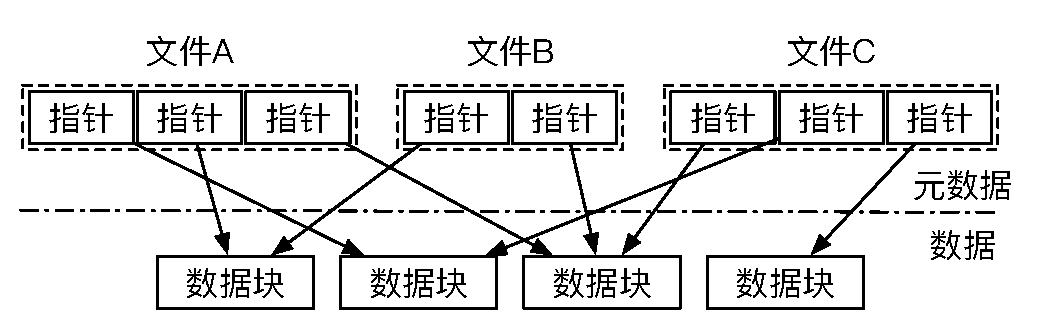
\includegraphics[width=0.75\textwidth]{pic/DedupSystemStorageMode.eps}
    \caption{数据重复数据删除系统的存储模式} 
    \label{fig:Deduplication-storage-pattern}
\end{figure} 

近年来,研究者提出加密后重复数据删除\cite{bellare2013MLE}以保护重复数据删除过程中的数据安全。图~\ref{fig:Cloud-based-encrypted-deduplication-storage-logic}描述了加密后重复数据删除系统框架,其包括客户端和云服务端两个主要组成部分。为了防止云服务商获取外包数据内容,加密后重复数据删除系统在客户端部署消息锁加密(MLE:message-locked encryption)\cite{bellare2013MLE}以加密明文数据块(简称为明文块),同时确保重复数据删除仍然能够作用于密文数据块(简称为密文块)以节约存储空间。传统对称加密算法为每个客户端或每个数据块分配不同加密密钥,导致相同的明文数据块被加密为不同的密文数据块,无法通过重复数据删除进行冗余消除。消息锁加密的核心思路时基于数据块内容产生密钥(称为MLE密钥,例如MLE密钥为明文数据块的哈希值\cite{douceur02}),从而将相同明文数据块加密为相同的密文数据块,以兼容直接针对密文数据块的重复数据删除。现有消息锁加密采用服务器辅助密钥生成方式(称为服务器辅助消息锁加密(Server-aided MLE)
\cite{keelveedhi2013DupLESS}),即部署第三方密钥服务器管理全局秘密,同时基于明文数据块哈希值以及密钥服务器的全局秘密共同生成MLE密钥,以防止攻击者针对MLE密钥实施离线暴力破解攻击。

\begin{figure}[!htb]
    \small
    \centering
    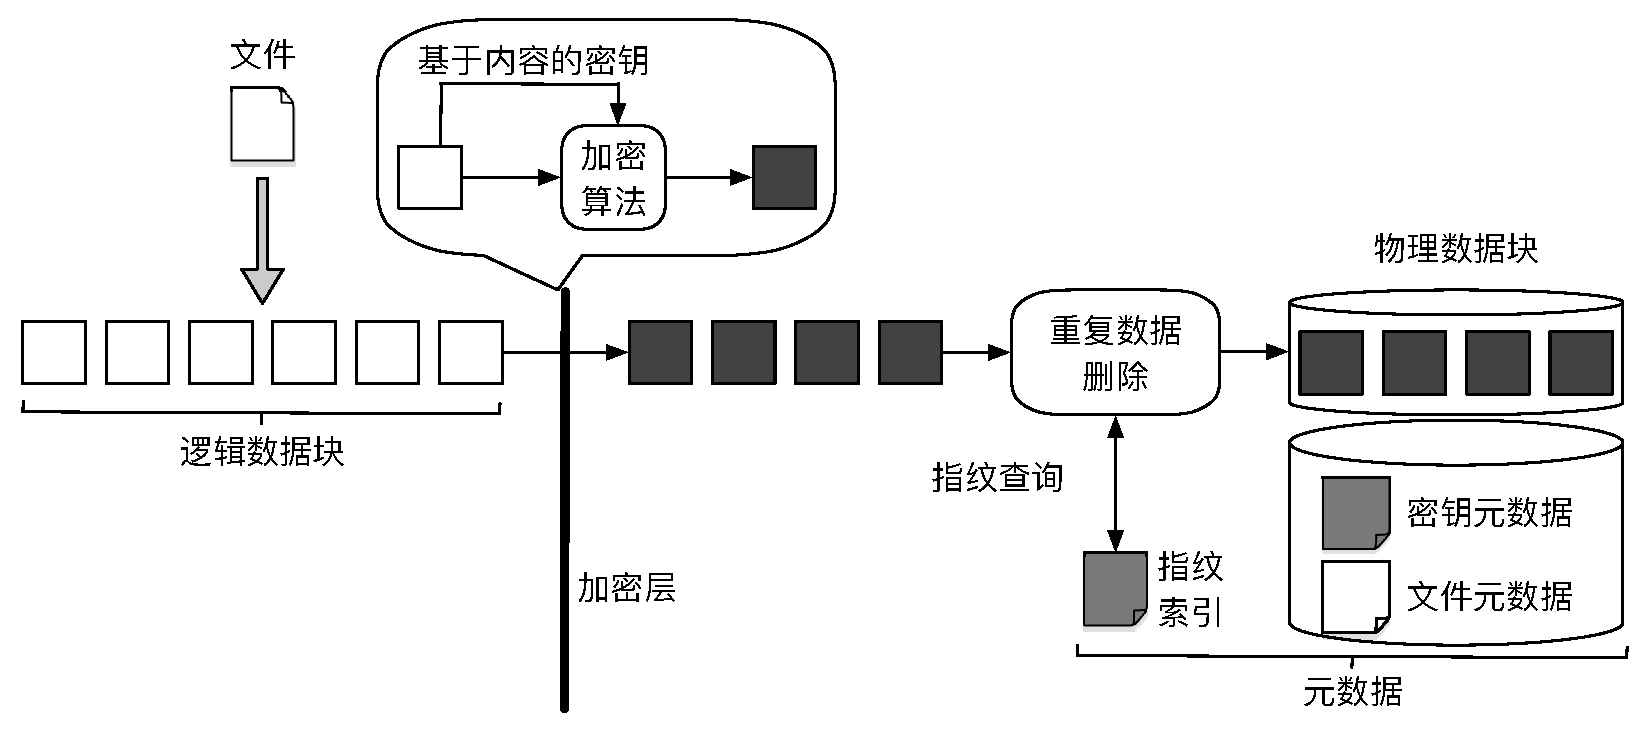
\includegraphics[width=\textwidth]{pic/EncryptDedupSystemLogic.eps}
    \caption{加密后重复数据删除系统逻辑视图}
    \label{fig:Encrypted-deduplication-storage-logic}
\end{figure}


传统对称加密为每个客户端分配独有密钥,导致来自不同客户端的相同明文块被加密为不同密文块,无法执行重复数据删除。消息锁加密的核心思想是基于数据块内容生成密钥(称为MLE密钥,例如MLE密钥为明文块的哈希值[14]),从而将相同明文块加密为相同密文块,以兼容直接针对密文块的重复数据删除。现有消息锁加密采用服务器辅助密钥生成方式(称为服务器辅助消息锁加密[8]),即部署第三方密钥服务器管理全局秘密,同时基于明文块哈希值以及密钥服务器的全局秘密生成MLE密钥,以防止攻击者针对MLE密钥实施离线暴力破解攻击。
\begin{figure}[!htb]
    \small
    \centering
    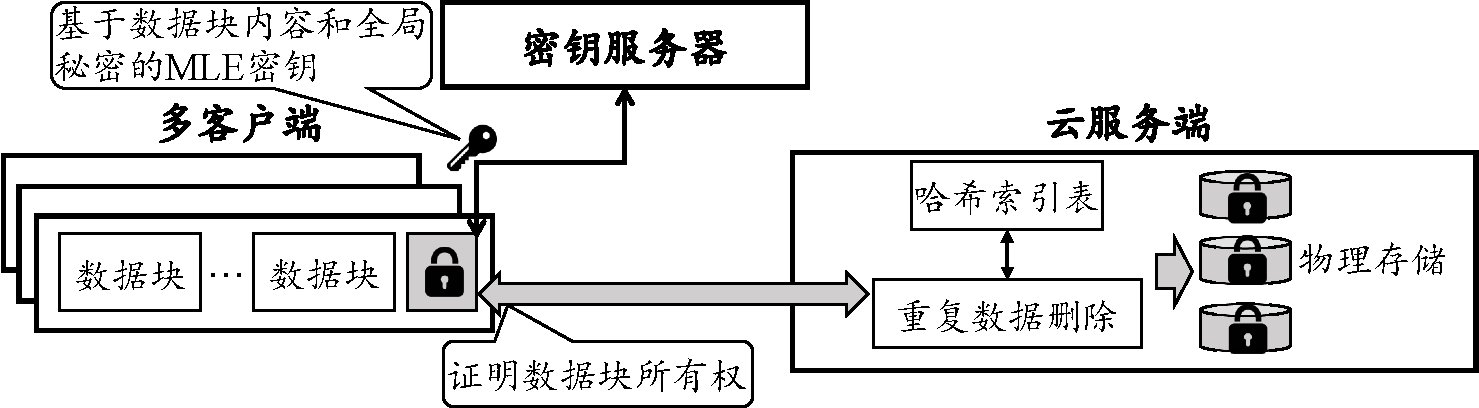
\includegraphics[width=\textwidth]{pic/Cloud-encrypted-deduplication-logic.pdf}
    \caption{面向云环境的加密后重复数据删除系统框架}
    \label{fig:Cloud-based-encrypted-deduplication-storage-logic}
\end{figure}
另一方面,重复数据删除受到伪造数据所有权的攻击威胁[20][31]。由于云服务商仅基于哈希值判断客户端是否拥有数据块,恶意用户/客户端可以伪造任意密文块的哈希值,如果该密文块已在云端存储(即发生重复数据删除),则恶意客户端无需传输密文块内容便可获得相应密文块的访问权限。
为了防止伪造所有权攻击,加密后重复数据删除增加了所有权证明(proof-of-ownership)技术[19]:除了密文块的哈希值以外,要求客户端额外提交目标密文块的所有权证明(proof);云服务商首先基于证明验证该客户端是否真实且完整拥有相应密文块,然后才执行如前所述的重复数据删除过程。所有权证明技术的合理性在于,只针对客户端真实拥有(即具有完整访问权限)的密文块执行重复数据删除,从而避免非法访问其他客户端的已存储内容。


\subsection{问题和动机}
\subsection{研究意义}

\section{国内外研究历史与现状}

\subsection{加密后重复数据删除}
\subsubsection{加密后重复数据删除技术}
\subsubsection{服务器辅助密钥生成}
\subsubsection{所有权证明技术}
\subsection{可信计算平台}
\subsubsection{Intel SGX}
\subsubsection{AMD SEV}
\subsubsection{ARM Trusted Zone}


\section{本文的主要贡献与创新}

\section{本论文的结构安排}